\documentclass[]{article}


\usepackage{xargs} 
\usepackage[colorinlistoftodos,prependcaption,textsize=tiny]{todonotes}
\newcommandx{\unsure}[2][1=]{\todo[linecolor=red,backgroundcolor=red!25,bordercolor=red,#1]{#2}}
\newcommandx{\change}[2][1=]{\todo[linecolor=blue,backgroundcolor=blue!25,bordercolor=blue,#1]{#2}}
\newcommandx{\info}[2][1=]{\todo[linecolor=OliveGreen,backgroundcolor=OliveGreen!25,bordercolor=OliveGreen,#1]{#2}}
\newcommandx{\improvement}[2][1=]{\todo[linecolor=purple,backgroundcolor=purple!25,bordercolor=purple,#1]{#2}}
\newcommandx{\thiswillnotshow}[2][1=]{\todo[disable,#1]{#2}}

\usepackage{graphicx}
\usepackage{auto-pst-pdf}
\usepackage{graphviz}
\usepackage{microtype}

%opening
\title{TinyRobo: An Affordable Tabletop Swarm Platform}
\author{Abraham Shultz}

\begin{document}

\maketitle

\begin{abstract}
Because simulations are necessarily incomplete, it is desirable to test algorithms for swarm robots on physical robots, rather than in simulation. 
However, the cost of robot hardware is high, and the larger a swarm, the more it will cost. 
This paper presents an inexpensive, open source hardware platform for converting toys into swarm robots, and a software infrastructure for controlling the swarm nodes. 
The resulting system was designed as a tabletop swarm, but has the ability to be expanded both in the area used by the swarm, and the capabilities of the individual swarm members. 

\end{abstract}

\section{Motivation}

Simulation of robots is clearly the lowest cost option for performing tests with large collections of robots. 
Once the simulation environment is created, adding additional robots does not cost more. 
Larger simulations may of course require more computer time, but by running at less than realtime, or improving the hardware the simulation runs on, this problem can be ameliorated. 

However, simulation brings with it a number of problems. 
Because simulations often can have bugs in them that are exploitable by agents operating in the simulation, it is sometimes possible to develop solutions that cannot be reproduced in reality. 
The use of genetic algorithms is particularly prone to these problems, as the genetic approach frequently develops ``solutions'' which solve the stated problem, but are not realistically useful. 
In one system, the fitness function for evolved simulated creature designs awarded high fitness to creatures that moved a long distance, quickly. 
This resulted in creatures that were very tall, and fell over as soon as the simulation started, resulting in a rapid horizontal movement as measured from the track of the creature's center of gravity over the ground \cite{brooks2000artificial, sims1994evolving}. 
A bug in the conservation of momentum in the same simulation resulted in creatures that moved by hitting themselves on the back. 

Additionally, simulations are often more perfect than the real world. 
In simulation, factors such as wheel slip, which adds error to robot odometry, and other forms of noise and sensor error can be left out of the simulation. 
Range limitations for sensors and communications can also be ignored, as distances in simulation are abstractions. 
These sorts of departures from reality are tempting, because they save processor time and development effort. 
With real hardware, these effects are included at no cost, and instead, substantial effort is put into minimizing them.

Unfortunately, crossing the gap from simulation to testing on real hardware requires the purchase of hardware, which can be a cause of substantial expense. 
This paper presents a hardware platform and the associated software framework to make a tabletop research robot swarm for about \$30 per robot. 
The hardware is designed to be adaptable to a wide variety of mobility platforms, and to accommodate the resulting changes with minimal alteration of the software controlling it. 

\section{Related Work}

\subsection{Overview of Previous Swarm Hardware}

Swarm robots are generally small. 
The reason to keep swarm robots small is related to both the cost of making them and the cost of using them. 
Larger robots consume more materials per unit, and so cost more money.
As a result, for a given number of swarm units, larger robots will result in a higher cost swarm. 
Also, each robot requires some amount of space to move around in. 
To keep the ratio of free space to robots constant, the area of space used by the robots grows as the robots do. 
If the ratio isn't kept constant, the robots will crowd each other, and so large robots will require either a very large space, or become overly crowded.
Finally, larger robots are just more cumbersome to deal with. 
They require larger storage areas, possibly teamwork to lift or repair, and so forth, all multiplied by the number of robots in the swarm. 

The robots used in most swarm work are of a sufficiently small size that many of them can fit in a room. In addition to budgetary constraints, interaction with an environment built for humans places an upper bound the scale of the individual swarm members. 
The lower bound on swarm robots is generally dictated by fabrication technology, with smaller robots becoming increasingly difficult to assemble. 
As a result of these bounds, swarm robots are mostly between 1cm$^3$ and 0.3m$^3$. 
This scale range can be divided into robots that can operate in swarms on a table, and those that can operate in swarms within a room, albeit possibly a large room. 
The challenge of construction of swarm robot hardware, then, is to put all of the same parts as non-swarm mobile robots: a mobility platform, a power supply, a processor, some sensors, and a communication system, into a small package.
Many impressive designs for small swarm robot platforms have been proposed and constructed as part of research in swarm robotics. 
However, most of these platforms are no longer easily commercially available, or never were. 


\subsubsection{Tabletop Swarms}

At the low end, in terms of size, the I-SWARM Project was intended to create a 2x2x1mm robot that moved by stick-slip locomotion actuated by piezo levers \cite{seyfried2005swarm}. 
Over the course of the project from 2004-2008, the hardware was developed and used in research, but was not converted to a commercial product.
Other techniques have been developed to use magnetic fields to apply force to small magnetic objects, resulting in controlled motion of the objects \cite{floyd2008untethered, pelrine2012diamagnetically}.
These systems are not amenable to decentralized control, because the moving components are not themselves robots. 
The moving parts are more accurately viewed as manipulators, with the instrumented environment and the manipulators themselves comprising a single robot. 

Alice, by Caprari et al. \cite{caprari1998autonomous} combined a PIC16F84 processor, motors, RF and IR networking, and enough battery power for 10 hours of autonomy into a robot measuring under 2.5cm$^3$. 
The processor used in Alice is relatively underpowered compared to modern processors at the same price point and power consumption. 
Alice robots are no longer available for purchase. 
The AmIR robot was similar to Alice in size and capability, but with a more modern processor \cite{arvin2009development}.
There is no evidence that AmIR was ever widely available.

The Jasmine swarm robots were possibly the closest thing to a commercially-available successor to Alice  \cite{kernbach2011swarmrobot}.
Jasmine measured 26x26x20mm, and included an ATMega processor, IR close range communication and obstacle detection, two motor skid steering, and li-po batteries.
Unfortunately, Jasmine units cost about 100 Euro (\$111 USD) each when they were available, and they are no longer available for purchase. 
The plans and information required to reproduce Jasmine units are available for free at Swarmrobot.org.
Assembling a Jasmine robot is not beyond the reach of competent electronics hobbyists, but it does require some unusual build processes, such as grinding down the cases of certain electronic parts and filling holes in the PCB with solder to prevent light leaks. 
The chassis of Jasmine is also a custom mechanical assembly, rather than a commercially available product. 

InsBot was a small robot, measuring 41mm x 30mm x 19mm, that was designed to interact with cockroaches \cite{colot2004insbot}.
It used two processors, one to run higher level behaviors and one to interface with a suite of sensors that included 12 IR sensors and a linear camera. 
InsBots were never commercially available, and each required approximately 6 hours of work to assemble by hand. 
However, the construction process appears to have been relatively straightforward. 

Even when they are commercially available, most existing swarm robots are too expensive to build a large swarm.
The Epuck from EFPL is approximately 800 Swiss francs (\$810 USD) per unit, so the cost of maintaining a large swarm can become daunting quickly. 
The high price of the Epuck is a result of its extensive suite of sensors, including a camera and 360$^{\circ}$ IR range sensor and communication system. 
Epucks also require a fairly smooth operating surface.
The Epuck uses differential drive, and allows the front or back edge of the robot to serve as a skid. 
Due to the relatively sharp corner of the lower edges of the robot, the Epuck can become stuck on 2-3mm high obstacles. 

The r-one research robot is cheaper than the Epuck, at approximately \$220 USD per unit \cite{mclurkin2013low}. 
The developers of the r-one position it as a more-featureful and less expensive alternative to the Epuck (\$810, cannot sense neighbors without additional hardware), Parallax's Scribbler (\$198, minimal sensors), the iRobot Create (\$220, requires additional hardware to be programmable), the K-team Khepera III (\$2000), and the Pololu 3pi (\$99, minimal sensors). The main advantage in sensing that the r-one has over these other platforms is neighbor sensors and ground truth position sensing, both of which are implemented on the r-one using infrared.
The design of the r-one is open source, but it does not appear to be commercially available as of this writing.   

The Harvard Kilobots are a more recent entry to inexpensive swarms, and have been produced in large quantities \cite{rubenstein2014kilobot}. 
Kilobots contain about \$15 worth of parts, but a 10-pack sells for 1100 Swiss francs, or about \$112 (US) per robot. 
The Kilobots are intended for research in a highly homogeneous environment, with most or all of the robots executing the same program. 
They are designed to be programmed in parallel using an IR interface. 
For small groups, individual Kilobots can be programmed differently, but any attempt to give each of a very large collection of robots an unique program will take a long time. 
The Kilobots move by stick-slip motion, and so must operate on a smooth surface, such as a whiteboard. 

One way to reduce the cost of swarm robots is to use commercial, off-the-shelf (COTS) hardware in the construction of the robot. 
Reusing existing hardware leverages the economies of scale that reduce the price of commercial hardware, as well as eliminating the need to design or build the COTS parts. 
Use of COTS parts in research robotics has led to at least two platforms referred to as COTSBots \cite{bergbreiter2003cotsbots, soule2011cotsbots}.
The first COTSBots used mote hardware for the communications link and sensing, plus a motor control add-on board \cite{bergbreiter2003cotsbots}. 
The mobility platform is a modified toy, in particular, a specific brand of high-quality micro RC car.
At the time of this writing, the car used in COTSBots is moderately expensive for a toy car, although quite cheap for a research robot, costing a little over \$100 (US) per unit. 
COTSBots use TinyOS, a modular and event-driven framework for developing node software \cite{levis2005tinyos}. 
TinyOS is written in a dialect of C called nesC. The motor and mote boards communicate using a messaging layer. 
The motor driver board is not commercially available, but can be custom-built by board fabrication companies, without the researcher having to assemble it by hand. 
The second COTSBots platform is larger, and will be discussed in the next section. 

\subsubsection{Room-sized Swarms}

One potential problem with extremely small swarms is that while the robots may scale down, the scale of obstacles they have to traverse may not scale with them. 
As previously mentioned, the Kilobots require a smooth surface, and the Epuck can be stopped by obstacles no more than a few millimetres tall. 
This sort of vulnerability prevents the smaller, tabletop swarm robots from operating well in human-scaled environments. 
In order to overcome this problem, larger swarm robots can be constructed.
 
The MarXbot swarm platform is capable of operating in unstructured human environments. 
MarXBots can also use their grippers to link themselves together and perform operations that an individual robot could not perform, such as bridging a gap larger than a single robot \cite{bonani2010marxbot}. 
The size and complexity of the MarXbots, as well as their powerful computer, renders the individual robots quite expensive. 

Swarmanoid extends the interlinking mechanism of MarXbot to a heterogeneous swarm with three different types of robots \cite{dorigo2013swarmanoid}.
The ``foot'' robots are MarXbots, and provide ground motion for ``hand'' robots. 
``Hand'' robots have grippers to manipulate objects, and can also climb.
The ``hand'' robots have an attachment point like the MarXbots, and so can be carried by ``foot'' robots. 
Flying ``eye'' robots provide overviews of the work area and networking.  

In order to reduce costs, another platform called COTSBots was developed \cite{soule2011cotsbots}.  
Instead of sensor motes on micro-scale RC cars, the newer COTSBots platform is composed of a laptop for processing and a modified RC car, tank, or similar toy as a mobility platform.
In order to interface between the laptop and motor drivers, a second micro-controller board, such as an Arduino or Phidget interface, may be used. 
Due to the diversity of possible combinations of hardware that can be assembled into this configuration, it is still a very viable platform. 
However, the minimum size of this style of COTSBot is the size of a laptop, which is in turn dictated largely by the minimum size of a useful keyboard. 
The large size of these COTSBots demands a very large space if the density of robots in a large swarm is to be kept low. 
Additionally, each laptop has a screen, keyboard, and so forth that are not useful while the robot is operating. 
All of these parts add to the overall cost of the swarm. 

Beyond the scale of rooms, swarm research has been done with Amigobots and Roombas, as well as larger custom platforms for outdoor multi-robot work \cite{guo2007bio, tammet2008rfid, olson2013cacm}.
In theory, swarm research could be performed using robots of any size, but financial limitations would place it out of the reach of most academic organizations. 

\section{Hardware}

The previously described swarm robot platforms tend to fall into one of two groups, from a hardware perspective. 
The first group uses microcontrollers and very limited onboard computation, but is small and relatively cheap.
This group includes Alice, Jasmine, AmIR, and the other tabletop systems. 
Due to their limited computation, these systems do not generally support complex algorithms such as vision processing. 
The second group use more powerful computers, but at a significant cost in weight, power consumption, and financial outlay.

The robot described in this work is intended to occupy a theoretical ``sweet spot'' at the high end of the tabletop swarms or the low end of the room-scale swarms, depending on how large of a mobility platform is used. 
As a result, if it is configured for tabletop operation, the system can be used with a minimum of available space. 
If, on the other hand, it is configured for room-scale operations, the system can be tested in natural or naturalistic human environments. 

The robot swarm developed for this work consists of a hardware module for controlling two motors of a toy, such as a small RC car, for mobility. 
The reasons for choosing this hardware design are explained in more detail below, but the overall intent is to have an inexpensive platform available for swarm research, without having to rely on any particular group of swarm robotics researchers starting and maintaining a side business supporting and selling robots.
Duplication of software and other digital artifacts is trivial, so constructing a duplicate of the hardware is the primary difficulty. 
The use of toys for the mechanical components of the robots is intended to reduce the difficulty of constructing the hardware. 
If researchers are not to be expected to become entrepreneurs, they should also not be expected to become expert machine tool operators.
The hardware resulting from this work is designed so that it can be duplicated by a researcher using common tools, and possessed of no more than hobby-level familiarity with electronic hardware.

\begin{figure}
\centering
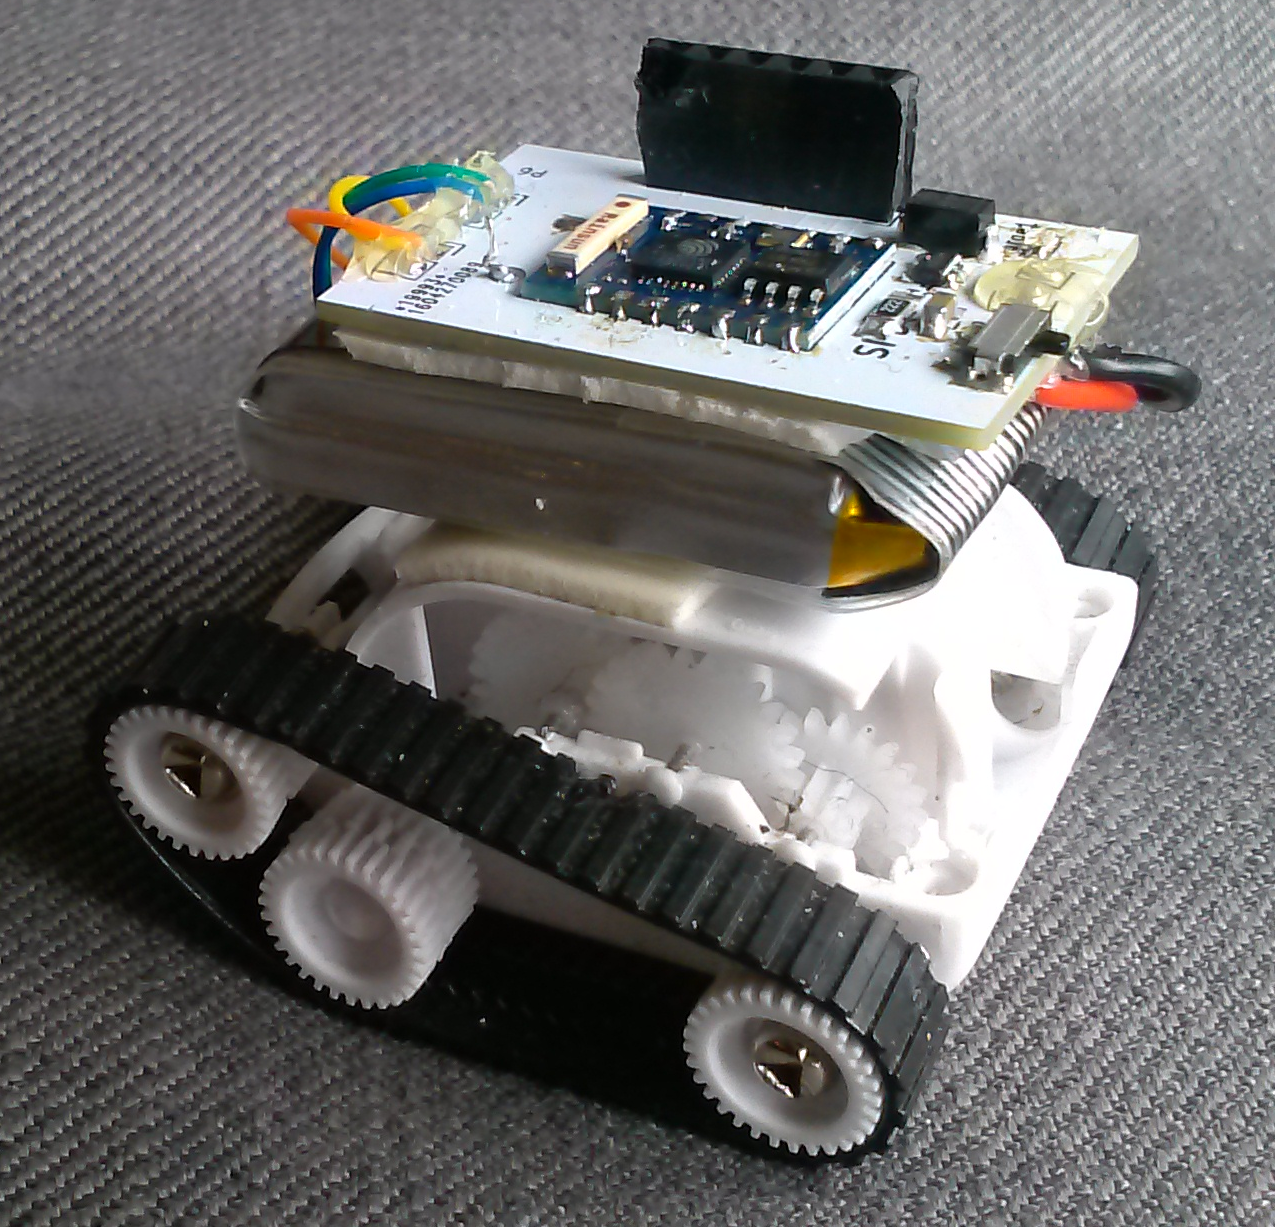
\includegraphics[width=0.8\textwidth]{../robot_makers_2/tiny_tank}
\caption{A tank-drive toy with a 3.7V lithium polymer battery and a TinyRobo control board mounted to it.}
\end{figure}

In order to be both heterogeneous and inexpensive, the robots used for this work are constructed by connecting a control hardware platform to children's toys. 
Modified toys are an adequate substitute for custom mechanical assemblies, and permit easy experimentation with heterogeneous swarms. 
The use of children's toys as mobility platforms may also avoid the sensitivity to the work surface exhibited by the Kilobots and, to a lesser extent, the Epucks.
The TinyRobo controller module was designed to be used as a replacement for the control electronics of children's toys, similar to the Spider-Bots developed by Laird, Price, and Raptis, or Bergbreiter's COTSBots \cite{lairdspider, bergbreiter2003cotsbots}.
However, unlike the Spider-Bots and COTSBots, TinyRobo does not specify a particular toy chassis to use for mobility. 
Most children's toys use either one motor with a mechanical linkage to cause the toy to turn when the motor is reversed, or two motors.
Two-motor toys frequently use either differential steering or have one motor provide drive power and the other provides steering. 
All of these toys can be controlled by the hardware described in this work. 

TinyRobos are intended to be heterogeneous, partly because of the advantages of heterogeneity in a swarm, and partly because toy supplies are unreliable.
While toys in the general case are expected to remain available, a particular line of toys might be discontinued or a modified version released. 
The software framework in development to support TinyRobos is based on ROS, and so allows modular replacement of the control algorithms used to convert desired motion of the robot into drive signals for the motors. 

%Toys cost $24, $16, $15, $21/2, 
\begin{table}
	\begin{tabular}{l l l l}
	Part & Price & Quantity & Subtotal\\
	\hline
	Mobile Toy & 14-20 & 1 & 20 \\
	Battery & 2.54 & 1 & 2.54 \\
	Main PCB & 2.75 &  1 & 2.75 \\
	ESP8266 Module & 2-7 & 1 & 7.0 \\
	DRV8830 & 2.30 & 2 & 4.60 \\
	MIC5319-3.3YD5 & 1.36 & 1 & 1.36 \\
	MCP73831 & 0.58 & 1 & 0.58 \\
	\hline
	Total & & & 27.83-38.83\\
	\end{tabular}
	\caption{All prices are for single quantities of new parts. It may be possible to get bulk discounts, especially on the toys and ESP-8226 modules. The costs of the resistors and capacitors has been left off, as they cost fractions of a penny each.}
\end{table}

The processor of the TinyRobo controller is an ESP-8266 wifi module.
The ESP-8266 costs approximately \$3-5, and contains both a wireless interface and a micro controller that can be programmed from a variety of programming environments and languages, including Lua and the Arduino variant of C/C++. The ESP-8266 module is based on the ESP-8266 IC, made by Expressif Systems. The IC itself has an 80Mhz Tensilica Xtensa L106 processor with 64kB of instruction memory and 96kB of data RAM. The modules come equipped with 512kB to 16MB of flash memory for program storage, and some combination of the 16 GPIO lines of the IC available for use. 
The ESP-8266 is available in several form factors, each designated by a different suffix. 
The version selected is the ESP-8266-03, which offers more GPIO pins than most other versions, and includes an internal antenna.

In addition to 802.11 b/g/n WiFi, the ESP-8266 supports a variety of serial protocols, including a UART, I$^2$C, and SPI. 
The I$^2$C interface is used on the TinyRobo board to connect to two DRV8830 motor driver ICs by Texas Instruments. 
The DRV8830 provides 1A of drive current.
Experimental tests with 8 different toys indicate that small toys draw well under 1A while moving freely, and peak around 2A when the motors are stalled. 
The tested toys include 3 insect-styled walkers, 3 wheeled vehicles (2 differential drive, 1 Ackerman steering), 1 toy helicopter, and 1 toy quadcopter.
The DRV8830 provides overcurrent limiting, so a stall condition or short circuit of the motor leads will disable the motor drive, but not damage the DRV8830. 


The TinyRobo control module also provides connections for a 3.7V lithium-ion battery pack, as well as charge control circuitry for the battery. 
The charge controller allows the TinyRobo to be charged from the same USB connection that is used to change the programming of the ESP-8266. 
Reset and entry into programming mode is controlled by a separate USB-to-serial adapter board, the Sparkfun BOB-11736.
Moving this functionality to the adapter board reduces the size and cost of the TinyRobo control module. 

\subsection{Toy Compatibility}

Children's toys normally use inexpensive brushed DC motors in their construction. 
These motors have not been the subject of extensive study, as they are commodity parts. 
However, it is useful to quantify their behavior to some extent, to determine which kinds of toys can be used with the TinyRobo controller. 

Two common types of motors found in children's toys are the RE and FA series of motors produced by Mabuchi Motor, or imitations of these motors produced by other companies. 
These motors use simple metal brushes and are constructed to be inexpensive, rather than precise. 
The intended voltage range of the motors varies with different winding types, but according to datasheets available from Mabuchi Motor, the voltage ranges and current draws for motors in this range are as shown in table \ref{tab:properBrandedMotors}.

\begin{table}
	\begin{tabular}{l l l l l}
	Model & Voltage & No Load Current & Max Efficiency & Stall Current\\
	\hline
	RE-140RA-2270 & 1.5-3 & 0.21 & 0.66 & 2.1 \\
	RE-140RA-18100 & 1.5-3 & 0.13 & 0.37 & 1.07 \\
	RE-140RA-12240 & 3-6 & 0.05 & 0.14 & 0.39 \\
	FA-130RA-2270 & 1.5-3 & 0.2 & 0.66 & 2.2\\
	FA-130RA-18100 & 1.5-3 & 0.15 & 0.56 & 2.1\\
	FA-130RA-14150 & 1.5-4.5 & 0.11 & 0.31 & 0.9\\
	\end{tabular}
	\caption{Current draw for Mabuchi-branded motors.}
	\label{tab:properBrandedMotors}
\end{table}

These are somewhat large brushed motors. 
For smaller toys, coreless motors are more common. 
The values in table \ref{tab:coreless} were measured from six of the toys used in constructing the TinyRobo swarm.
The measurements from the toy helicopter and toy quadcopter are included for comparison.
While the TinyRobo board can supply sufficient current to control all of these toys, it has not been tested in flying platforms.

\begin{table}
	\begin{tabular}{l l l}
	Motor number & No Load Current & Stall Current (measured)\\
	\hline 
	Hexbug brand mini spider & 0.03A & 0.13A* \\
	Hexbug brand 6-legged insect & 0.06A & 0.25A \\
	Miniature toy RC car & 0.21A & 0.8A \\
	Miniature toy RC insect & 0.19A & 1.13A \\
	Miniature toy RC vehicle & 0.37A & 0.8A \\
	Miniature toy RC vehicle & 0.06A & 0.74A \\
	Toy helicopter & 0.07A & 1.12A \\
	Toy quadcopter & 0.74A & 1.99A \\
	\end{tabular}
	\caption{No load and stall current for coreless DC micromotors. Measurements were performed at 3V supply voltage. * The Hexbug mini spider includes a slip clutch, so attempting to stall the motors by holding the toy still does not prevent the motor from turning}
	\label{tab:coreless}
\end{table}


\subsection{Potential for Expansion}

The current design for TinyRobo does not include sensors as a cost-saving decision. 
However, the communication between the ESP-8266 and the motor drivers uses the industry standard I2C bus serial interface. 
Due to the non-proprietary nature of this interface standard, it has been widely adopted, and many sensors are available to connect to an I2C bus. 
For example, Vishay Semiconductor makes the VCNL3020, which is an infrared proximity sensor with a 20mm range. 
If greater range is required, The ST Microelectronics VL53L0X Time-of-flight (ToF) laser ranger and gesture sensor provides a 2M range and 1D gesture sensing in a 4.4mm x 2.4mm package. 
As of this writing, the VCNL3020 is \$3.44 and the VL53L0X costs \$6.28 in single quantities.
These prices are reduced significantly when buying components in bulk, but because they increase the cost, size, and power draw of the hardware, they have not yet been integrated with the TinyRobo platform. 
Numerous multichannel ADC ICs with I2C interfaces are also available, which permits the addition of analog sensors to the TinyRobo platform. 

\section {Firmware}

The current version of the TinyRobo firmware is developed in the open-source Arduino development environment.
Arduino programs are written in a dialect of C++. 

Every robot runs the same firmware. 
The firmware listens for connections on port 4321 for TCP/IP packets containing one of two types of messages. 
Messages starting with a 0x51 byte (ASCII 'Q') cause the firmware to respond with a message containing the ASCII string "TinyRobo". 
This function is to allow automatic detection of TinyRobos on a network by querying all connected systems to determine if they respond in this way. 

Messages starting with a 0x4D byte (ASCII 'M') followed by four bytes are motor speed commands.
The firmware interprets the first two bytes as the speed and direction for the first motor, and the second two bytes as speed and direction for the second motor.
The control bytes are converted to a single byte command for the DRV8830 driver and transmitted over the I2C bus to set the motor speed.
 
The DRV8830 driver is a voltage-controlled motor driver. 
It accepts a single-byte command for each motor. 
Bits 7-2 of the byte define the output voltage to be applied to a motor, and the driver attempts to maintain that output voltage.
The valid range of motor voltage commands for the DRV8830 driver is 0x06 to 0x3F, which corresponds to a range of 0.48V to 5.06V in 0.08V increments. 
Because the TinyRobo battery is nominally 3.7V, the motor command 0x30 is the highest output available. 
Bits 1 and 0 of the command byte control the polarity of the output voltage, and so the direction of the motor, as per table \ref{tab:DRV8830_truth}.

\begin{table}
	\begin{tabular}{l l l l l}
	Bit 1 & Bit 0 & Out 1 & Out 2 & Function\\
	\hline
	0 & 0 & Z & Z & Coast\\
	0 & 1 & L & H & Reverse\\
	1 & 0 & H & L & Forward\\
	1 & 1 & H & H & Brake\\				
	\end{tabular}
	
	\caption{Truth table for DRV8830 drive direction bits. Coast allows the motor to turn freely. Brake connects the motor leads, which results in braking using the motor's back-EMF}
	\label{tab:DRV8830_truth}
\end{table}

Once the motor speed is set, the firmware reads the fault bytes from the DRV8830, and sends the motor command and the fault bytes for each motor back to the client over WiFi. 
The client uses the fault bytes to detect overcurrent conditions in the motor drivers and reduce output power. 

The decision to have all of the robots have the same firmware and control the speed of the motors from ROS was made because different toys have different control schemes. 
Toy tanks use differential drive, toy cars have Ackerman steering, and so forth. 
By moving the control to the main computer, the firmware can be kept simple while still allowing researchers to adapt the system to the available toys. 

\section{Software}

The TinyRobo swarm is controlled by ROS nodes running on a single computer.
Since all of the robots are controlled by a single computer, it may appear that this is a highly centralized system. 
However, the central computer provides a framework for implementing a decentralized control scheme on the individual robots. 

%Graphic of the software environment as a whole
\begin{figure}
	\centering
	\digraph[scale=0.6]{Framework}{
	
	graph[nodesep=0.5];

	subgraph clusterRobot1 {
		motor[shape=box; label="Motor Driver"];
		robotCode[label=<Robot <br/> Firmware>];
		robotCode -> motor;
		label="Robot 1";
		shape=box;
	}
	
	subgraph clusterRobot2 {
		motor2[shape=box; label="Motor Driver"];
		robotCode2[label=<Robot <br/> Firmware>];
		robotCode2 -> motor2;
		label="Robot 2";
		shape=box;
	}
	
	subgraph clusterRobot3 {
		motor3[shape=box; label="Motor Driver"];
		robotCode3[label=<Robot <br/> Firmware>];
		robotCode3 -> motor3;
		label="Robot 3";
		shape=box;
	}
	
	subgraph clusterRobotN {
		motorN[shape=box; label="Motor Driver"];
		robotCodeN[label=<Robot <br/> Firmware>];
		robotCodeN -> motorN;
		label="Robot N";
		shape=box;
	}
	
	subgraph clusterComp {
		concentrate=true;
		label="Control Computer";
		{rank=source;
			aprilTag [label="Tag Detector"];
		}
		
		{rank=same;
			vrLaser [label="Laser Service"];
			vrNet [label="Network Service"];
			vrDist [label="Distance Service"];			
		}
		
		{rank=same rp1 rp2 rp3 rpN}
		
		rp1 [label=<Robot <br/> Process 1>];
		rp2 [label=<Robot <br/> Process 2>];
		rp3 [label=<Robot <br/> Process 3>];
		rpN [label=<Robot <br/> Process N>];
		lc1 [label=<Robot 1<br/> Laser>];
		lc2 [label=<Robot 2<br/> Laser>];
		//vrNet -> {rp1, rp2, rp3, rpN} [dir="both"];
		//vrSense -> {rp1, rp2, rp3, rpN};
		
		//Distance informs whether robots can be reached on the net
		vrNet -> vrDist;
		vrDist -> vrNet;
		
		rp1 -> robotCode [label="WiFi", dir="both"];
		rp2 -> robotCode2 [label="WiFi", dir="both"];
		rp3 -> robotCode3 [label="WiFi", dir="both"];
		rpN -> robotCodeN [label="WiFi", dir="both"];
	
		//Robots 1 and 2 have laser clients getting scans
		lc1 -> vrLaser;// [label=<std\string_msgs/Integer>];
		vrLaser -> lc1;// [label=<sensor\string_msgs/LaserScan>];
		lc1 -> rp1;
		lc2 -> vrLaser;// [label=<std\string_msgs/Integer>];
  		vrLaser -> lc2;// [label=<sensor\string_msgs/LaserScan>];
		lc2 -> rp2;
		
		//Robots 3 and N are talking over the network
		rp3 -> vrNet;
		vrNet -> rpN;
					
		//April tags inform distance and laser
		aprilTag -> vrDist;// [label=<apriltags\string_ros/TagDetections>];	
		aprilTag -> vrLaser;// [label=<apriltags\string_ros/TagDetections>];
		
				
	}
	
	camera[label=<Overhead<br/>Camera>;shape=box;]
	camera->{vrLaser, aprilTag};	
		 
	}
	\caption{Overview of the framework. Rectangular nodes are hardware, oval nodes are software. Robots 1 and 2 have virtual lasers, robots 3 and N are communicating over the network.}
\end{figure}

Rather than all of the robots being controlled by a single program on the central computer, each robot has ROS nodes that are responsible for controlling that robot. 
Each of these nodes only has access to the information that would be available to that robot, and so acts as if it is a local control program running on the robot.
However, since the ROS nodes are running on a relatively modern desktop PC, they have substantial processing power available to them. 
As a result, the individual robots are small, lightweight, and consume relatively little electrical power, but still have significant computing power. 
As more powerful and lower power consumption processors become available, more of the processing can be moved from the central computer and onto the actual robots, enabling a smooth transition from a simulated decentralized system to a real decentralized system. 

Individual TinyRobos have minimal sensing capacity, due to their small size. 
The central computer has a top-down camera over the ``arena'' the TinyRobos are active in. 
Each TinyRobo has an AprilTag \cite{olson2011tags} on top of it, so that the central computer can localize them within the arena. 
The central computer uses the location information to create ``virtual sensors'' for each robot. 
Since the central computer knows the location of each robot, the relevant information can be sent to each robot's control process as if it were coming from a sensor on the robot. 

For example, since the central computer knows the location, adding a range and bearing sensor that allows each robot to detect the distance and angle of the nearby robots is simple to implement. 
This functionality is available in hardware on Epucks and Marxbots, but since each robot must be equipped with it, the cost scales linearly with the number of robots to equip.  

It is possible to calculate the odometry for individual robots by watching the change in position in their tags over time. 
The calculated odometry could then be published as a ROS topic, just like odometry collected from e.g. wheel encoders. 
This functionality has not been implemented yet, but would be useful for testing distributed SLAM algorithms on the swarm. 

The virtual sensors can also be configured to emulate error conditions such as noisy sensors, failed sensors, degraded localization, and so forth.
Virtual parameter tweaking will allow fine-grained testing of the behavior of algorithms under imperfect conditions, and the response of human users to unreliability in the swarm. 

\subsection{Virtual Localization}

The AprilTag tracking of the robots provides localization of the robots within a common coordinate frame. 
It should be stressed that while the central computer can localize the robots, both relative to each other and by absolute position within the arena, this information may be withheld from the individual robots, or given to them if required. 
The code virtually operating on the robot may be neither aware of its own position in the world, nor the location of other robots, if the experiment calls for such a lack of information. 

Currently, the AprilTag-based localization is used to implement virtual laser scanners similar to the Sick or Hokoyu brand laser scanners used on larger robots. 
It is also used to limit the range of messages sent between the robots through a virtual network. 

\subsection{Virtual Laser Scanners}

The AprilTag localizations and the image of the arena are used to provide virtual laser rangers for each robot. 
The virtual laser ranger consists of two ROS nodes, a service and clients for the service. 
The service is called ``laser\_oracle\_server''. 
It subscribes to the AprilTag detections and the images from the arena overhead camera. 
 
When a client requests a laser scan, the virtual laser service masks the modified arena image with a circle with a radius of the laser range, centered on the robot requesting the scan.
This masking removes all of the objects that are out of range of the laser, and so reduces the time spent calculating the laser scan points. 

Each sample of the laser scan is represented as a line segment, located based on the requested start, stop and inter-measurement angles for the virtual laser scanner. 
Each line segment is checked for intersection with the lines defining the contours of the blue objects in the image. 
As the virtual laser service receives images, it draws a blue dot over the location of every robot. 
This dot provides the outer edge of each robot in the virtual laser scan. 
The approach of using blue objects as obstacles was chosen because if the laser scanner service treats anything blue as an obstacle, then ``walls'' can be created in the arena by making lines of blue masking tape on the arena floor. 
If multiple intersections are found for a line segment, the intersection closest to the robot is used, as the laser would stop after reflecting off an object.
The service then formats the distances to the intersection points as a ROS sensor\_msgs/LaserScan and returns it as the service response to the requesting client. 

The virtual laser clients take the place of the laser driver ROS nodes that would be used to control a real linear laser scanner. 
The laser client is initialized with some parameters, such as the sweep angle and angular resolution of the virtual laser, and polls the laser service regularly. 
As it receives laser scans from the service, it publishes them to a ROS topic in the same manner as a ROS node for a hardware laser. 

The apriltags\_ros node publishes the detected locations of the tags in meters, but the computer vision detection of blue objects in the arena camera image operates in pixels. 
In order to convert from pixels to real-world distances, the apriltags\_ros node was forked and a modified version was created that provides the locations of the tags in pixel as well as real-world coordinates. 
The modified version is available at https://github.com/ab3nd/apriltags\_ros.

\begin{figure}
	\centering
	\digraph[scale=0.6]{VirtualLaserSystem}{
	
	vls -> vsc [label=<std\string_msgs/Integer&nbsp;&nbsp;&nbsp;&nbsp;>];
	vsc -> vls [label=<sensor\string_msgs/LaserScan>];
	vsc -> sub1 [label=<sensor\string_msgs/LaserScan>];
	cam -> vls [label=<sensor\string_msgs/Image>];
	cam -> atag	[label=<sensor\string_msgs/Image>];
	atag -> vls [label=<apriltags\string_ros/TagDetections>];	
		 
	vls [label="Virtual Laser Service"];
	vsc [label="Virtual Laser Client"];
	atag [label="AprilTag Detector"];
	cam [label="Arena Camera"];
	sub1 [label="Subscriber"];
	}
	\caption{Data flow in the virtual laser service}
\end{figure}

\subsection{Virtual Networking}

If the robots are required to communicate directly with each other, the communication passes through a virtual network.
From the point of view of the robots, messages sent into the virtual network are delivered to other robots as if the messages were sent directly from one robot to another. 
However, all the communication is taking place between processes running on the central computer.
By changing how the messages are delivered by the central system, the virtual network can provide full connectivity, range-limited mesh networking, directional beacons, or other forms of networking. 
The reliability of the network can also be varied, by dropping some messages or otherwise changing them based on information about the robots. 
For example, the likelihood that a message arrives at the robot to which it was transmitted may depend on the distance between the sender and receiver. 

\begin{figure}
	\centering
	\digraph[scale=0.6]{VirtualNetwork}{
	
	{rank=same atag dist}
	{rank=same tx rx}

	vns -> dist [label="Robot IDs"];
	dist -> vns [label="Distance"];
	cam -> atag	[label=<sensor\string_msgs/Image>];
	atag -> dist [label=<apriltags\string_ros/TagDetections>];	
	vns -> rx [label="Network Message"];
	tx -> vns [label="Network Message"];	 
	
		
	vns [label="Virtual Network Service"];
	dist [label="Distance Service"];
	atag [label="AprilTag Detector"];
	cam [label="Arena Camera"];
	tx [label="Transmitter"];
	rx [label="Receiver"];
	}
	\caption{Data flow in the virtual network. The virtual network service can take the distance between the transmitting robot and the receiving robot into account when determining if the message is delivered.}
\end{figure}


\section{Conclusions}

Swarm software is frequently described as centralized or decentralized. 
In a centralized system, a single computer coordinates the actions of the swarm by commanding each individual robot. 
In a decentralized system, robots use their local processors and sensor information to make control decisions. 
The TinyRobo design works with ROS to provide an emulation of a decentralized system within a centralized system. 
While this paper presents it in the context of a complete system, the software framework is not tightly bound to the TinyRobo hardware, and so may be useful to other users of tabletop swarms. 

The combination of hardware and software presented in this work makes it possible to construct swarm robots at a cost of around \$30 per robot. 
The resulting robots are useful for swarm robotics research, and the price point is accessible to many institutions, as well as private individuals. 
All of the software used is open source, and available for no cost. 

\bibliography{../proposal/swarm.bib}
\bibliographystyle{apalike}

 
%\change{More detail on the motors used in children's toys. Quantify the behavior of a bunch of motors.}

%For tables \ref{tab:FA-series}, \ref{tab:RE-series}, and \ref{tab:coreless}, the motor current at stall was estimated by applying a regulated 3.3v supply to the motor and measuring the voltage drop across the motor. 

%This was done to avoid damage to the motors. 
%In toys, the current to the motors is frequently limited by the available current from the batteries, and stalling the motor is prevented by simple slip clutches or play in the motor drive train. 

%\change{Add photos of motors, with cm scale for visual clairity}
%\change{Two main types of motors, ~2cm$^3$ brushed DC and >1cm$^3$ coreless motors}

%\begin{table}
%	\begin{tabular}{l|l|l}
%	Motor number & No Load Current & Stall Current (estimated)\\
%	2 & 0.08 &
%	3 & 0.35 &
%	4 & 0.02 &
%	5 & 0.11 &
%	6 & 0.20 &
%	7 & 0.02 &
%	8 & 0.33 &
%	\end{tabular}
%	\caption{No load and stall current for Mabuchi FA series and similar motors. Measurements were performed at 3.3V supply voltage. Motor 1 was defective.}
%	\label{tab:FA-series}
%\end{table}


%\begin{table}
%	\begin{tabular}{l|l|l}
%	Motor number & No Load Current & Stall Current (estimated)\\
%	\end{tabular}
%	\caption{No load and stall current for Mabuchi RE series and similar motors. Measurements were performed at 3V supply voltage.}
%	\label{tab:RE-series}
%\end{table}

\end{document}
